\documentclass[12pt,a4paper]{article}
\usepackage[utf8]{inputenc}
\usepackage[polish]{babel}
\usepackage{amsmath}
\usepackage{amsfonts}
\usepackage{times}
\usepackage[T1]{fontenc}
\setlength{\parindent}{0.5cm}
\usepackage{url}
\usepackage{hyperref}
\usepackage{breakurl}
\usepackage{algorithm}
\usepackage{algpseudocode}
\usepackage{graphicx}
\usepackage{subfig}
\usepackage{csvsimple}
\graphicspath{ {./resources/} }
\pagenumbering{gobble}

\author{Jakub Mazur, Maciej Purski}
\title{Kolorowanie grafów za pomocą metod heurystycznych (SK16) - GIS sprawozdanie 2}


\begin{document}
\maketitle

\section{Temat projektu}

\indent
Projekt ma na celu implementację algorytmu rozwiązującego problem kolorowania grafu.
Przez kolorowanie rozumiemy podział zbioru wierzchołków $V$ na $k$ rozłącznych klas $C_k$ w taki
sposób, że jeśli dowolne dwa wierzchołki $u$ i $v$ należą do jednej klasy $C_k$ , to wierzchołki te nie
są połączone krawędzią.

Celem algorytmu będzie wyznaczenie takiego podziału na klasy, by liczba $k$ była jak
najmniejsza oraz, by nie występowały konflikty tj. nie można było znaleźć dwóch wierzchołków
połączonych krawędzią, które byłyby w jednej klasie.
Do rozwiązania problemu zostanie wykorzystana metoda heurystyczna \textbf{przeszukiwania z tabu}.

\section{Algorytm}

\textbf{Przeszukiwanie z tabu} jest heurystyczną metodą służącą do rozwiązywanie problemów optymalizacyjnych. Opiera się na przeszukiwaniu lokalnego sąsiedztwa danego rozwiązania. Tego typu metody posiadają silną tendencję do zatrzymywania się w optimum lokalnym. Algorytm przeszukiwania z tabu zakłada przechowywanie pewnego zbioru ostatnio odwiedzonych rozwiązań, tak aby przeszukiwanie nie \textit{utknęło} w optimum lokalnym.

Algorytm może być używany do różnego typu problemów optymalizacyjnych. Jego postać ogólna została przedstawiona w \cite{alhe-tabu}. Dla zastosowania algorytmu do rozwiązania problemu kolorowania grafu, należy uszczegółowić jego poszczególne elementy, co jest tematem kolejnych podrozdziałów.

\subsection{Reprezentacja rozwiązania}
\textit{Rozwiązaniem} będziemy nazywali podział zbioru wierzchołków \textit{V} na \textit{k} niepustych podzbiorów, które można interpretować jako \textit{klasy} lub \textit{kolory}.

\subsection{Warunki początkowe}
Początkowa liczba kolorów $k$ będzie stanowiła parametr algorytmu. Wierzchołki zostaną pokolorowane w sposób losowy z gwarancją, że każdy z $k$ kolorów zostanie użyty co najmniej raz - czyli innymi słowy zbiór wierzchołków grafu zostanie podzielony na $k$ niepustych podzbiorów. Takie początkowe kolorowanie nie musi być wcale kolorowaniem poprawnym.


\subsection{Sąsiedztwo}
Zgodnie z \cite{coloring} \textbf{sąsiednim} rozwiązaniem $y\in N(x)$ do rozwiązania $x$, nazywamy takie rozwiązanie \textit{y}, które można uzyskać poprzez zmianę przynależności jednego z wierzchołków rozwiązania \textit{x}. Generacja jednego sąsiada polega na wylosowaniu jednej z niepustych klas $C_i$, następnie wylosowaniu wierzchołka $v\in C_i$ oraz liczby $j\in\langle1,k\rangle$, gdzie $k$ to liczba klas. Następnie wierzchołek $v$ jest kolorowany na kolor $j$. Jeżeli wylosowano tę samą klasę, do której należy wierzchołek, losowanie jest powtarzane.

W każdym kroku generowane jest $g$ sąsiadów \textit{punktu roboczego}\footnote{tj. aktualnie przetwarzanego}, gdzie $g$ stanowi parametr algorytmu. Spośród zbioru sąsiadów wybierany jest najlepszy element względem funkcji kosztu, który nie należy do listy tabu. Będzie on nowym punktem roboczym.

\subsection{Lista tabu}
W naszym projekcie skorzystamy z metody zarządzania oraz reprezantacji listy tabu przedstawionej w artykule \cite{Hertz1987}. Lista tabu zostanie zaimplementowana jako kolejka FIFO o rozmiarze $n$ zadanym jako parametr algorytmu. Będzie ona przechowywała zakazane \textit{ruchy}. \textit{Ruchem} nazywamy zmianę wierzchołka \textit{v} z koloru \textit{i} na kolor \textit{j}. W każdej iteracji algorytmu wybierany jest najlepszy ruch (pod względem wartości funkcji celu), który nie znajduje się na liście tabu. Stworzy on nowy punkt roboczy. Na listę trafi natomiast ruch \textit{odwrotny} do wykonanego, a zatem będzie to para składająca się z wierzchołka \textit{v} oraz koloru \textit{i}, będącego \textit{starym} kolorem. Kiedy lista tabu się zapełni, zostanie z niej usunięty ostatni element.

\subsection{Funkcja kosztu}
Aby możliwe było porównywanie poszczególnych rozwiązań, należy zdefiniować funkcję kosztu, która ma być zminimalizowana przez algorytm przeszukiwania z tabu. Pochodzi ona z artykułu \cite{coloring}. Ma ona postać:

\begin{equation}
\label{cost}
cost(x) = - \sum_{i=1}^{k}|C_i|^2 + \sum_{i=1}^{k} 2\cdot|C_i|\cdot|E_i|
\end{equation}

gdzie $C_i$ oznacza $i$-tą klasę kolorowania, natomiast $E_i$ oznacza zbiór konfliktujących krawędzi w tej klasie. Pierwszy człon tej funkcji (pierwsza suma) odpowiada za minimalizację liczby klas poprzez \textit{premiowanie} jak najbardziej licznych klas. Drugi człon zas odpowiada za minimalizację liczby konfliktujących krawędzi.


Jedną z głównych obserwacji odnośnie tej funkcji, przedstawionych we wspomnianym artykule, jest to, że jej
minima lokalne odpowiadają podziałom bez konfliktów. Należy zauważyć, że liczba $k$ zawarta we
wzorze nie zakłada z góry ilości użytych kolorów. Minimalizacja liczby użytych kolorów będzie niejako
„efektem ubocznym” minimalizacji wartości funkcji celu.


\subsection{Kryterium stopu}
Algorytm nie ma naturalnego kryterium stopu. Jedną z możliwości, na którą zdecydowaliśmy się w naszej implementacji jest zatrzymanie algorytmu po zadanej liczbie iteracji $t$, która jest parametrem agorytmu.

\subsection{Parametry}
Reasumując, algorytm będzie przyjmował następujące parametry:
\begin{itemize}
\item Początkowa liczba kolorów
\item Liczba iteracji
\item Rozmiar sąsiedztwa
\item Rozmiar listy tabu
\end{itemize}


\section{Implementacja}
Algorytm zostanie zaimplementowany w języku C++. Będzie on odczytywał graf w formie tekstowej ze standardowego wejścia i wypisywał rozwiązanie na standardowe wyjście. Możliwe będzie wypisywanie historii wartości funkcji kosztu aktualnego punktu roboczego w celu zbadania jej zmienności w ciągu kolejnych iteracji algorytmu oraz wypisanie najlepszego znalezionego rozwiązania.

Do automatyzacji procesu ewaluacji rozwiązania posłuży skrypt w języku Python, który będzie powtarzał eksperymenty odpowiednią liczbę razy oraz rysował wykresy obrazujące zmianę wartości funkcji kosztu.

\subsection{Struktury danych}
\subsubsection{Reprezentacja grafu}
Graf zostanie zaimplementowany jako \textbf{macierz sąsiedztwa}. Z punktu widzenia naszego algorytmu istotna jest bowiem możliwość sprawdzania w czasie stałym, czy dana krawędź istnieje. W tym celu użyta zostanie klasa \textit{boost::adjacency\_matrix} z bilbioteki \textit{Boost Graph}.

\subsubsection{Lista tabu}
Lista tabu zostanie zaimplementowana jako bufor cykliczny o stałym rozmiarze, który umożliwia dodawanie elementów na koniec oraz usuwanie z początku w czasie stałym. Do implementacji listy tabu zostanie użyta klasa \textit{boost::circular\_buffer} z biblioteki \textit{Boost Container}.

\subsubsection{Punkt roboczy}
Punkt roboczy, czyli aktualnie najlepsze rozwiązanie będzie reprezentowany jako \textit{wektor klas}, gdzie \textit{klasą} nazywamy podzbiór wierzchołków. Liczba klas $k$ jest stała, w wektorze są zatem przechowywane także takie klasy, które są puste. \textit{Klasa} składa się z listy wierzchołków do niej należących oraz liczby konfliktów w danej klasie.

\newpage
\subsection{Pseudokod}
\label{ssec:pseudo}

\begin{algorithmic}

\State $G\gets odczytaj()$

\State $x\gets zainicjujPunktRoboczy(k)$
\Comment parametr k - początkowa liczba klas

\State $globalnieNajlepszy \gets x$
\State $tabu\gets zainicjujListeTabu(t)$
\Comment parametr t - rozmiar listy tabu

\State $i\gets 0$
\While {$i < iters$}
\Comment parametr iters - liczba iteracji

\State $ruchyVek \gets zainicjujWektorRuchow()$
\For {$j\gets0; j < N; j++$}
\Comment Generacja losowych sasiadow
\State $cPocz \gets rand(0, k)$
\State $v \gets rand(0, nWierzcholkow(cPocz))$
\State $cKon \gets rand(0, k)$
\State $ruchyVek.push\_back(cPocz, v, cKon)$
\EndFor

\State $najlepszyDot \gets null$
\For {$ g \in ruchyWek$}
\Comment Wybór najlepszego sąsiada
\If {$koszt(x, g) < koszt(x, najlepszyDot) \;\textbf{and}\; g\; \textbf{not in}\; tabu$}
\State {$najlepszyDot \gets g$}
\EndIf
\EndFor

\State {$x.wykonajRuch(najlepszyDot)$}
\State {$tabu.dodajRuchOdwrotny(najlepszyDot)$}
\State {$i++$}

\If{$koszt(x) < koszt(globalnieNajlepszy)$}
\State{$globalnieNajlepszy \gets x$}
\EndIf

\EndWhile
\State {Zwróć $globalnieNajlepszy$}
\end{algorithmic}

Powyższy pseudokod opisuje ogólne działanie algorytmu. Zaniedbane są pewne szczegóły w tym obliczanie funkcji kosztu na podstawie wzoru \ref{cost}. Możliwa jest optymalizacja tej funkcji poprzez obliczanie jedynie zmiany jej wartości po wykonaniu potencjalnego ruchu. Wiadomo, że wartość $|C_{cPocz}|$ spadnie o 1 a wartość $|C_{cKon}|$ wzrośnie o 1. Liczba konfliktów wewnątrz klasy zmieni się także jedynie dla klas $cPocz$ oraz $cKon$. Aby sprawdzić o ile zmniejszy się wartość $|E_{cPocz}|$ wystarczy policzyć ile wierzchołków z tej klasy konfliktowało z wierzchłkiem $v$. Podobnie dla $E_{cKon}$ wystarczy policzyć ile wierzchołków byłoby w konflikcie z wierzchołkiem $v$ po dodaniu go do klasy.


\section{Badanie rozwiązania}
\subsection{Dobór parametrów}
Przed rozpoczęciem właściwych eksperymentów i oceny efektywności rozwiązania, konieczne jest określenie optymalnych wartości parametrów tj. przede wszystkim długości listy tabu oraz rozmiaru sąsiedztwa. Parametry te zostaną ustalone doświadczalnie – algorytm zostanie uruchomiony dla kilku standardowych przypadków grafów, np. grafu losowego $G_{n,p}$\footnote{Jest to graf losowy, generowany według modelu Erdősa–Rényi \cite{erdos59a}, gdzie $n$ oznacza ilość wierzchołków, natomiast $p$ oznacza prawdopodobieństwo, że dowolna z możliwych krawędzi zostanie włączona do grafu.} z różnymi wartościami parametrów. Pozwoli to ustalić, dla jakich wartości parametrów algorytm działa efektywnie.

\subsection{Optymalizacja funkcji kosztu}
Ważnym elementem oceny rozwiązania jest zbadanie, jak zmienia się wartość funkcji kosztu wraz z kolejnyi iteracjami. Aby można było zbadać jej zmienność w ciągu kolejnych iteracji, program będzie logował wartości funkcji celu w kolejnych iteracjach. Dane te zostaną zebrane w formie wykresów. Pozwoli to sprawdzić, czy wartość funkcji zbiega do minimum, a także, ile iteracji jest do tego potrzebne.

\subsection{Ewaluacja rozwiązania}
\label{ssec:eval}
Najważniejszym kryterium ewaluacji rozwiązania dla konkretnego przypadku grafu \textit{G} będzie uzyskana liczba chromatyczna \textit{k}. Aby można było w sposób miarodajny określić efektywność implementacji, należy przetestować algorytm na wielu różnorodnych przypadkach grafów. W tym celu zostaną wykorzystane standardowe grafy wykorzystywane w wielu artykułach traktujących o tematyce kolorowania grafów. Doskonały przegląd tych grafów, a także wyników uzyskanych przez najlepsze algorytmy można znaleźć w \cite{article}.

Dla potrzeb ewaluacji rozwiązania algorytm zostanie uruchomiony na przypadkach grafów opisanych we wspomnianym artykule. Uzyskana liczba chromatyczna oraz czas działania i liczba iteracji programu zostaną porównane z wynikami przedstawionymi w artykule.

\section{Eksperymenty}
Zostały przeprowadzone dwie fazy eksperymentów: badanie parametrów oraz poszukiwanie najlepszych rozwiązań - jako najlepsze uznajemy rozwiązanie o jak najniższej liczbie chromatycznej bez konfliktów. Eksperymenty polegały na wielokrotnym uruchamianiu algorytmu dla różnych rodzajów grafów, przy kilku zestawach parametrów startowych. Podczas eksperymentów wykorzystano zestaw grafów stworzonych na potrzeby konkursu \textit{The Second DIMACS Implementation Challenge}\cite{Johnson}. Dotyczył on implementacji algorytmów rozwiązujących problemy NP-trudne na grafach, m.in. problem kolorowania wierzchołków. Powstały dla celów konkursu zbiór problemów obejmuje grafy o różnej budowie, dlatego świetnie nadaje się do przetestowania przygotowanej implementacji.

\subsection{Zmienność funkcji kosztu}

Na rysunku (1) widoczna jest zmienność kosztu aktualnie najlepszego kolorowania. Poziomą żółtą linią oznaczono na wykresach wartość minimalną uzyskaną przez algorytm. Dla grafów większych zbieżność jest znacznie wolniejsza (widoczne na trzech pierwszych wykresach). Na dwóch ostatnich wykresach widoczna jest \textit{skokowość} zmian wartości funkcji kosztu.


\begin{figure} [H]

\begin{tabular}{cc}
\subfloat{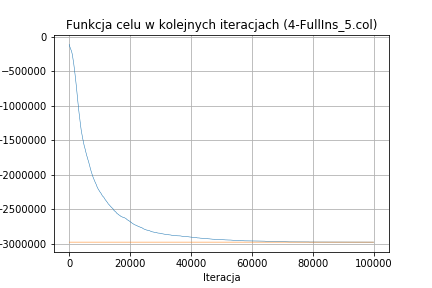
\includegraphics[width = 2.8in]{Release/4full5}} &
\subfloat{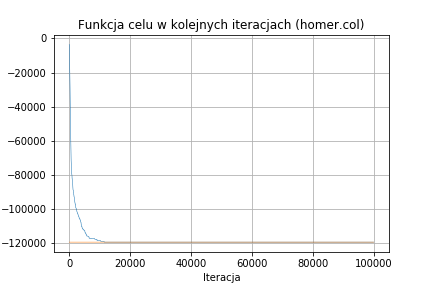
\includegraphics[width = 2.8in]{Release/homer}} \\
\subfloat{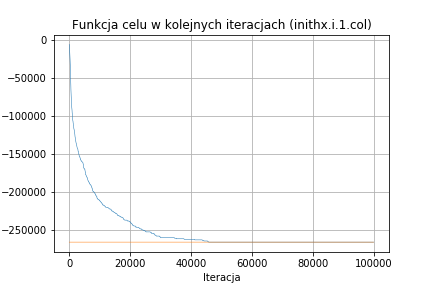
\includegraphics[width = 2.8in]{Release/inithx1}} &
\subfloat{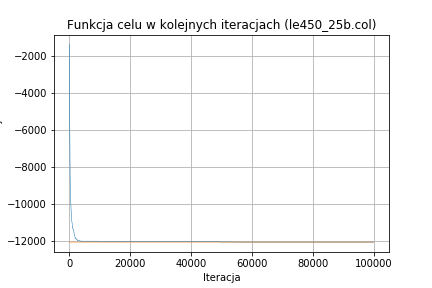
\includegraphics[width = 2.8in]{Release/le450}} \\
\subfloat{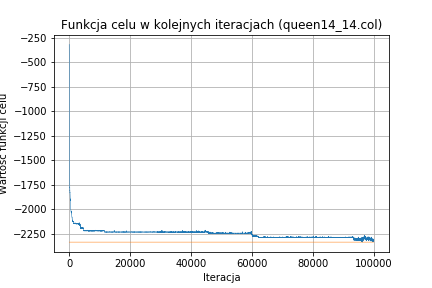
\includegraphics[width = 2.8in]{Release/queen}} &
\subfloat{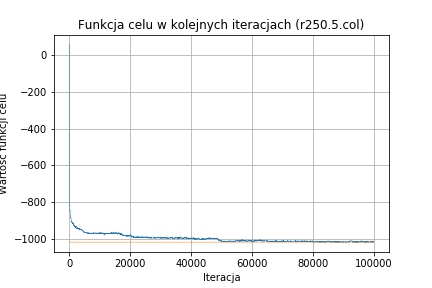
\includegraphics[width = 2.8in]{Release/r250}} \\


\end{tabular}

\caption{Badanie zmienności funkcji kosztu na różnych grafach}
\end{figure}

\subsection{Badanie parametrów}
Badaniom podlegało zachowanie algorytmu względem rozmiaru sąsiedztwa oraz rozmiaru listy tabu. Celem badania było sprawdzenie, czy rozmiar sąsiedztwa i długość listy tabu zależą silnie od charakterystyki konkretnego grafu. Poszukiwany był taki zestaw parametrów, który byłby na tyle ogólny, by dało się go zastosować do dowolnego grafu, którego charakterystyka nie jest znana. 

\subsubsection{Rozmiar sąsiedztwa}
Na rysunkach (2) oraz (3) przedstawiono badanie rozmiaru sąsiedztwa. Aby sprawdzić, jak rozmiar sąsiedztwa wpływa na działanie algorytmu, z różnych rodzin grafów wybrano po kilku przedstawicieli. Rozmiar sąsiedztwa był wyznaczany jako iloczyn liczby wierzchołków i pewnego współczynnika. Wartości tego współczynnika zmieniały się w zakresie $<0.1, 1.0>$, z krokiem równym $0.1$. Na każdy współczynnik przyjęto 10 lub 6 uruchomień algorytmu. Otrzymywana liczba kolorów była zapisywana do logu, by następnie wyznaczyć minimalną, maksymalną i średnią liczbę kolorów uzyskaną przy danym współczynniku. Długość listy tabu pozostawała niezmienna, natomiast początkowa liczba kolorów stanowiła około $0.4$ liczby wierzchołków.

\begin{figure} [H]

\begin{tabular}{cc}
\subfloat{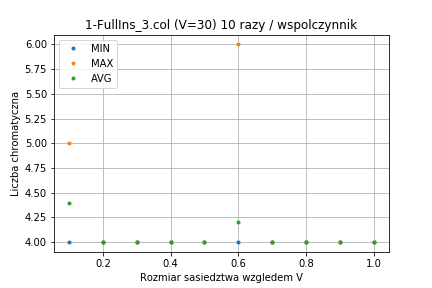
\includegraphics[width = 2.8in]{1-FullIns3}} &
\subfloat{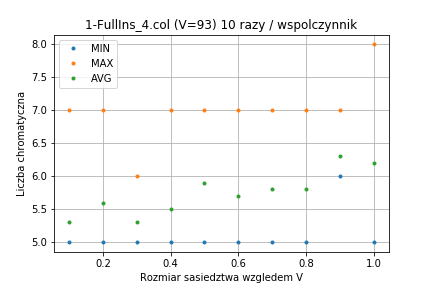
\includegraphics[width = 2.8in]{1-FullIns4}} \\
\subfloat{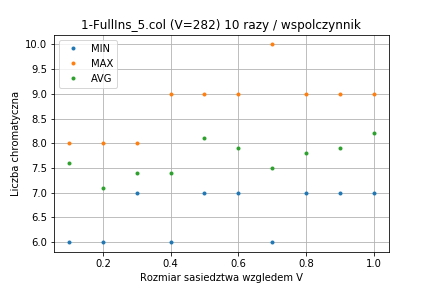
\includegraphics[width = 2.8in]{1-FullIns5}} &
\subfloat{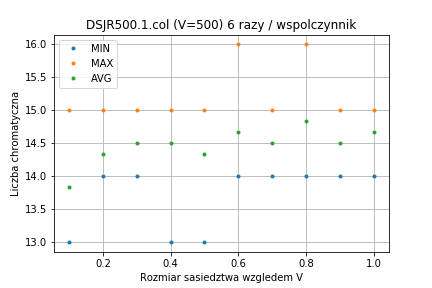
\includegraphics[width = 2.8in]{DSJR500}} \\
\subfloat{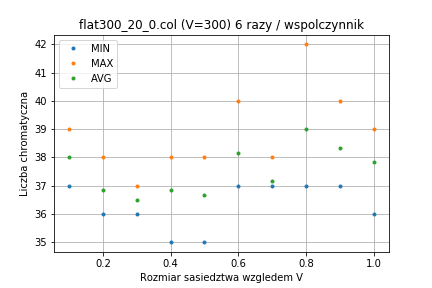
\includegraphics[width = 2.8in]{flat300}} &
\subfloat{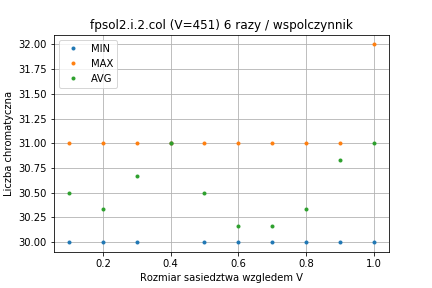
\includegraphics[width = 2.8in]{fpsol2}} \\
\subfloat{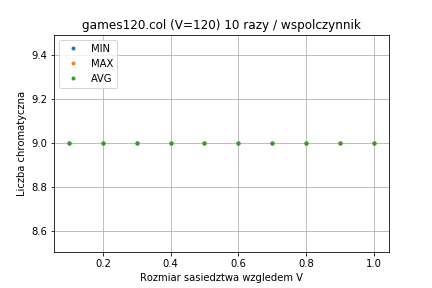
\includegraphics[width = 2.8in]{games120}} &
\subfloat{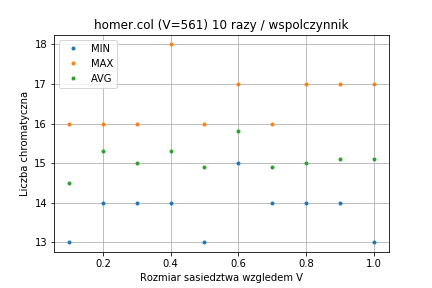
\includegraphics[width = 2.8in]{homer}} \\

\end{tabular}

\caption{Badanie rozmiaru sąsiedztwa}
\end{figure}

\begin{figure}  [H]
\begin{tabular}{cc}

\subfloat{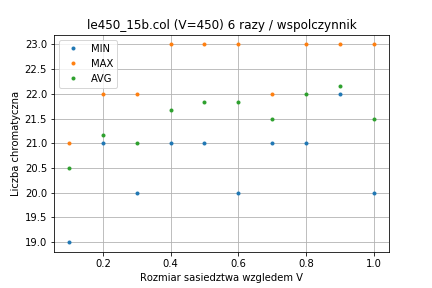
\includegraphics[width = 2.8in]{le450}} &
\subfloat{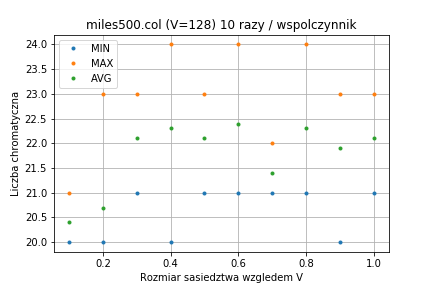
\includegraphics[width = 2.8in]{miles500}} \\
\subfloat{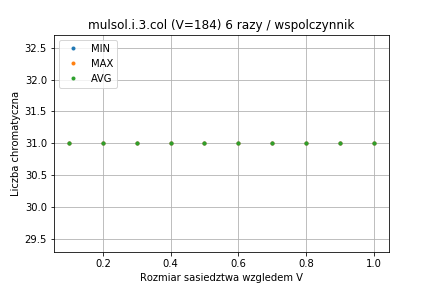
\includegraphics[width = 2.8in]{mulsol}} &
\subfloat{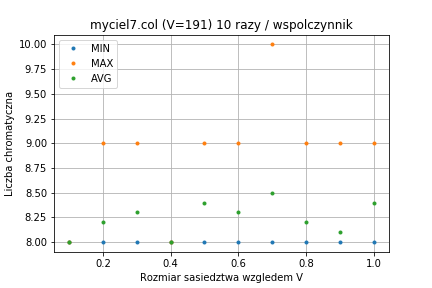
\includegraphics[width = 2.8in]{myciel7}} \\
\subfloat{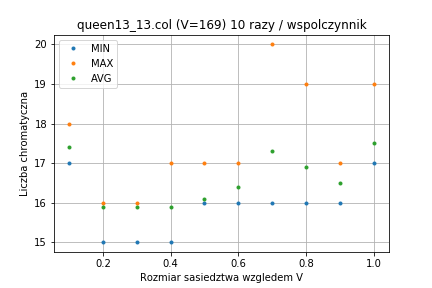
\includegraphics[width = 2.8in]{queen13}} &
\subfloat{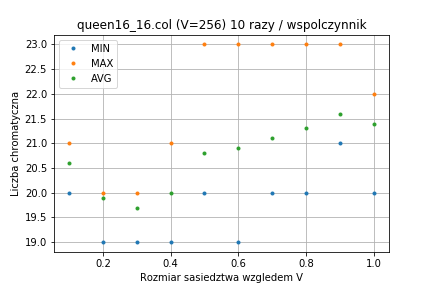
\includegraphics[width = 2.8in]{queen16}} \\
\subfloat{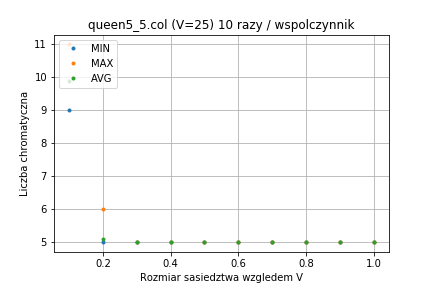
\includegraphics[width = 2.8in]{queen5}} &
\subfloat{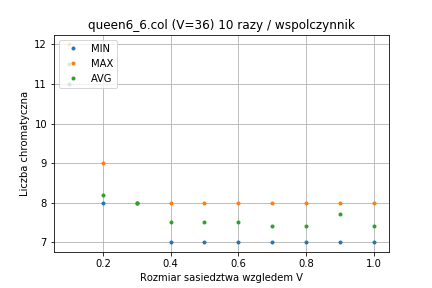
\includegraphics[width = 2.8in]{queen6}} \\

\end{tabular}
\label{n2}
\caption{Badanie rozmiaru sąsiedztwa c.d.}
\end{figure}

Zgodnie z przewidywaniami, w większości przypadków rozmiar sąsiedztwa miał duży wpływ na zwracaną liczbę kolorów. Jak można zaobserwować na wykresach, usilne zwiększanie rozmiaru nie owocowało znaczącą poprawą rozwiązania. Przeciwnie, w wielu przypadkach zarówno średnia jak i minimalna liczba kolorów stawały się coraz gorsze wraz ze wzrostem sąsiedztwa. Z analizy wyników można odczytać, że rozmiary sąsiedztwa nie przekraczające wartości $0.5 V$ sprawdzały się najlepiej. Należy jednak zauważyć, że optymalny współczynnik, dający najmniejszą średnią liczbę kolorów jest mocno zależny od konkretnego przypadku grafu.

Na podstawie wyników eksperymentu, w trakcie wykonywania poszukiwań liczby chromatycznej, opisanych w kolejnych rozdziałach, jako optymalny rozmiar sąsiedztwa przyjęto wartość około $0.5$. Potwierdzenie tej wartości można też odnaleźć w \cite{Hertz1987}.

Warto również wspomnieć, że rozmiar sąsiedztwa bardzo silnie wpływa na czas wykonania programu. Z tego właśnie powodu, rozpoczynanie poszukiwań z dużym sąsiedztwem może okazać się nieopłacalne.

\subsubsection{Badanie rozmiaru listy tabu}
Badanie wpływu rozmiaru listy tabu przebiegało analogicznie do badania rozmiaru sąsiedztwa. Podobnie jak poprzednio, dla różnych rodzajów grafów uruchamiano algorytm z kilkoma długościami listy tabu. Długości te pochodziły ze zbioru $\lbrace7,10,20,40,100\rbrace$. Dla każdej długości tabu uruchomiono algorytm 5 razy, za każdym razem logując zwracaną liczbę kolorów. Wyniki w postaci minimalnej, maksymalnej i średniej liczby kolorów zaprezentowano na wykresach widocznych na rysunkach (4) oraz (5). Pozostałe parametry, tj. początkowa liczba kolorów i rozmiar sąsiedztwa ustalono odpowiednio na $0.4V$ i $0.5V$.

\begin{figure}  [H]
\begin{tabular}{cc}

\subfloat{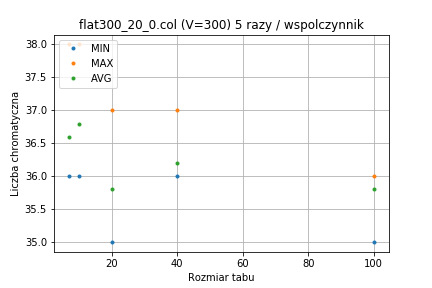
\includegraphics[width=2.8in]{tabu/flat300}} &
\subfloat{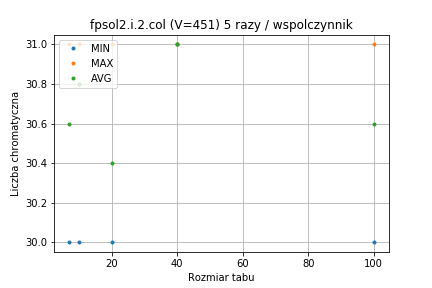
\includegraphics[width=2.8in]{tabu/fpsol2}} \\
\subfloat{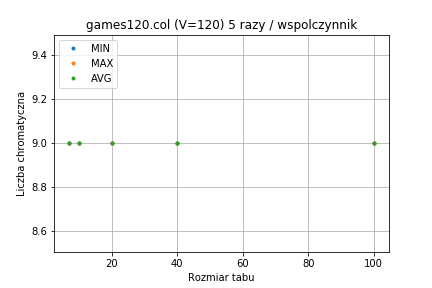
\includegraphics[width=2.8in]{tabu/games120}} &
\subfloat{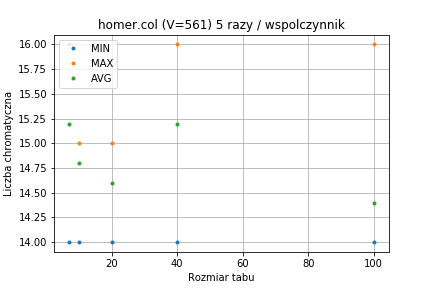
\includegraphics[width=2.8in]{tabu/homer}} \\
\subfloat{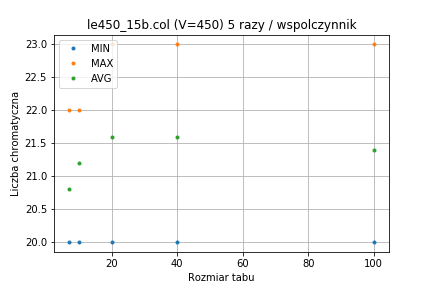
\includegraphics[width=2.8in]{tabu/le450}} &
\subfloat{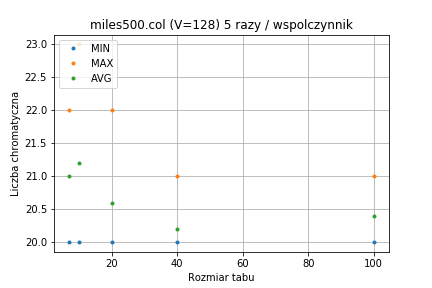
\includegraphics[width=2.8in]{tabu/miles500}} \\
\subfloat{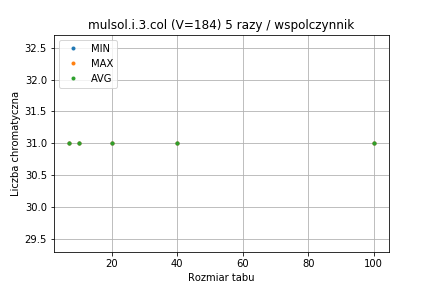
\includegraphics[width=2.8in]{tabu/mulsol}} &
\subfloat{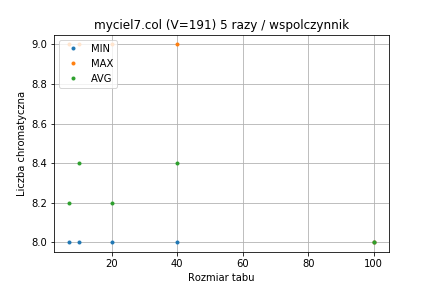
\includegraphics[width=2.8in]{tabu/myciel7}} \\

\end{tabular}
\label{fig:t1}
\caption{Badanie rozmiaru tabu}
\end{figure}

\begin{figure}  [H]
\begin{tabular}{cc}

\subfloat{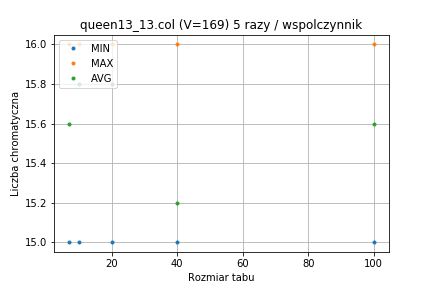
\includegraphics[width=2.8in]{tabu/queen13}} &
\subfloat{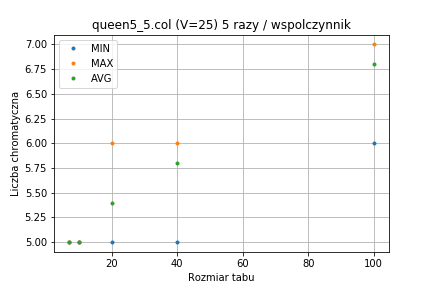
\includegraphics[width=2.8in]{tabu/queen5}} \\
\subfloat{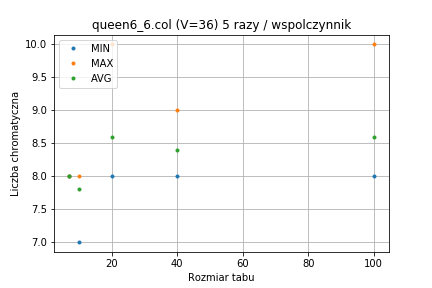
\includegraphics[width=2.8in]{tabu/queen6}} & 
\subfloat{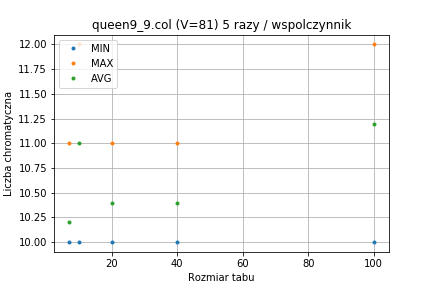
\includegraphics[width=2.8in]{tabu/queen9}} \\

\end{tabular}
\label{fig:t1}
\caption{Badanie rozmiaru tabu c.d.}
\end{figure}

Podobnie jak w przypadku rozmiaru sąsiedztwa, długość listy tabu w większości przypadków miała wpływ na zwracaną liczbę kolorów. Analiza wyników wskazuje, że krótsze listy tabu generują lepsze rezultaty. Obserwując wszystkie wykresy można zauważyć, że tabu o długości 7 niemal w każdym wypadku zwróciło minimalną liczbę kolorów. Wartość ta jest również postulowana w \cite{Hertz1987}. Z tego powodu, do wyznaczania liczby chromatycznej w kolejnych rozdziałach przyjęto listę tabu o długości 7.
\subsubsection{Początkowa liczba kolorów}
Ważnym elementem algorytmu jest początkowa liczba kolorów. Oczywistym jest, że aby algorytm odnalazł kolorowanie bez konfliktów, liczba ta nie może być mniejsza od rzeczywistej liczby chromatycznej grafu. Zazwyczaj jednak nie posiadamy dobrego oszacowania tej liczby. Testy algorytmu wykazały jednak dużą odporność na początkową liczbę kolorów tj. nawet startując od liczby kolorów wprost równej liczbie wierzchołków, algorytm jest w stanie znacząco zredukować liczbę użytych kolorów.

W przypadku rozważanych tutaj grafów, liczby chromatyczne były dokładnie znane. Z tego też powodu, dla celu automatyzacji przeprowadzanych testów, przyjęto bezpieczną wartość $0.4 V$, która w każdym przypadku była większa od liczby chromatycznej.

Należy tutaj zauważyć, że początkowa liczba kolorów ma istotne znaczenie dla zmiany ciężaru pomiędzy eksploracją i eksploatacją przestrzeni rozwiązań. Duża liczba możliwych kolorów będzie wywierać presję w stronę eksploracji. Wynika to ze sposobu generowania sąsiedniego rozwiązania, które w swoim ostatnim kroku przypisuje wierzchołkowi losowy kolor z zakresu 1 do k.

Temat balansu pomiędzy eksploracją i eksploatacją oraz dobierania początkowej liczby k zostanie jeszcze omówiony w rozdziałach prezentujących wyniki poszukiwań liczby chromatycznej dla testowanych grafów.

\subsection{Wyniki poszukiwań liczby chromatycznej}
Jak opisano w poprzednich rozdziałach, na potrzeby testów wykorzystano zbiór grafów przygotowanych dla konkursu DIMACS. Aby ocenić poprawność przygotowanej implementacji, dokonano porównania z wynikami klasycznych algorytmów (m.in. DSATUR i RLF) przedstawionymi w artykule \cite{article}.
W artykule tym również wykorzystano grafy z konkursu DIMACS. Zbiór testowanych grafów został podzielony na kilka grup, różniących się charakterystykami :
\begin{itemize}
\item Grafy Mycielskiego i SGB - w tej grupie można znaleźć klasyczne grafy Mycielskiego oraz grafy ze Stanford GraphBase (SGB), reprezentujące m.in. połączenia między miastami w USA (grafy \textit{miles}) czy też relacje pomiędzy postaciami danej książki (grafy \textit{david}, \textit{jean}, \textit{anna}, \textit{homer}, \textit{huck}),
\item grafy queens - grafy w których wierzchołki reprezentują pola szachownicy, natomiast krawędzie dodawane są tylko wtedy, gdy królowe postawione na polach odpowiadających wierzchołkom atakują się wzajemnie,
\item grafy CAR - grafy inspirowane grafami Mycielskiego, jednak trudniejsze w kolorowaniu,
\item grafy losowe i flat - trudne algorytmicznie grafy losowe stworzone przez Davida Johnsone'a, oraz grafy flat zaproponowane przez Culbersone'a,
\item grafy RAC - reprezentują rzeczywisty problem alokacji zmiennych z kodu pośredniego do rejestrów procesora przez kompilator,
\item grafy Leighton - każdy z nich składa się z 450 wierzchołków. Cechą charakterystyczną jest zmieniająca się liczba chromatyczna przy niezmiennej gęstości.
\end{itemize}

Dla każdego grafu opisanego w artykule uruchamiano algorytm od 10 do 15 razy, z następującymi parametrami: 
\begin{itemize}
\item $c = 0.4V$
\item $n = 0.5V$
\item $t = 7$
\item \begin{equation}
    i =
    \begin{cases}
      250 000, & \vert V \vert < 500 \\
      500 000,& \vert V \vert >= 500
    \end{cases}
  \end{equation}
\end{itemize}
Następujące tabele prezentują najlepsze uzyskane wyniki, porównane z rzeczywistą liczbą chromatyczną oraz wynikami algorytmów opisanymi w artykule.

\begin{figure} [H]
\begin{tabular}{|c|c|c|c|c|c|}%
	\hline
    \bfseries Graf & V & E & Faktyczne $\chi$ & Najlepsze $\chi$ z artykułu & \bfseries Tabu $\chi$
    \csvreader[head to column names]{resources/queensResults.csv}{}% use head of csv as column names
    {\\\hline \Graph & \V & \E & \Chrom & \ArticleBest & \bfseries\TabuBest}% specify your coloumns here
    \\ \hline
\end{tabular}
\caption{Pomiary dla grafów typu queens}
\end{figure}

\begin{figure} [H]
\begin{tabular}{|c|c|c|c|c|c|}%
	\hline
    \bfseries Graf & V & E & Faktyczne $\chi$ & Najlepsze $\chi$ z artykułu & \bfseries Tabu $\chi$
    \csvreader[head to column names]{resources/leightonResults.csv}{}% use head of csv as column names
    {\\\hline \graph & \v & \e & \chrom & \art & \bfseries\tabu}% specify your coloumns here
    \\ \hline
\end{tabular}
\caption{Pomiary dla grafów Leightona}
\end{figure}

\begin{figure} [H]
\begin{tabular}{|c|c|c|c|c|c|}%
	\hline
    \bfseries Graf & V & E & Faktyczne $\chi$ & Najlepsze $\chi$ z artykułu & \bfseries Tabu $\chi$
    \csvreader[head to column names]{resources/mycielResults.csv}{}% use head of csv as column names
    {\\\hline \graph & \v & \e & \chrom & \art & \bfseries\tabu}% specify your coloumns here
    \\ \hline
\end{tabular}
\caption{Pomiary dla grafów Mycielskiego}
\end{figure}

\begin{figure} [H]
\begin{tabular}{|c|c|c|c|c|c|}%
	\hline
    \bfseries Graf & V & E & Faktyczne $\chi$ & Najlepsze $\chi$ z artykułu & \bfseries Tabu $\chi$
    \csvreader[head to column names]{resources/racResults.csv}{}% use head of csv as column names
    {\\\hline \graph & \v & \e & \chrom & \art & \bfseries\tabu}% specify your coloumns here
    \\ \hline
\end{tabular}
\caption{Pomiary dla grafów rac}
\end{figure}  
    
\begin{figure} [H]
\begin{tabular}{|c|c|c|c|c|c|}%
	\hline
    \bfseries Graf & V & E & Faktyczne $\chi$ & Najlepsze $\chi$ z artykułu & \bfseries Tabu $\chi$
    \csvreader[head to column names]{resources/randomResults.csv}{}% use head of csv as column names
    {\\\hline \graph & \v & \e & \chrom & \art & \bfseries\tabu}% specify your coloumns here
    \\ \hline
\end{tabular}
\caption{Pomiary dla grafów losowych}
\end{figure}  

\begin{figure} [H]
\begin{tabular}{|c|c|c|c|c|c|}%
	\hline
    \bfseries Graf & V & E & Faktyczne $\chi$ & Najlepsze $\chi$ z artykułu & \bfseries Tabu $\chi$
    \csvreader[head to column names]{resources/car.csv}{}% use head of csv as column names
    {\\\hline \graph & \v & \e & \chrom & \art & \bfseries\tabu}% specify your coloumns here
    \\ \hline
\end{tabular}
\caption{Pomiary dla grafów car}
\end{figure}  

\subsection{Wnioski}
Jak wynika z analizy wyników, algorytm uzyskał bardzo dobre wyniki dla szerokiej gamy grafów. W większości przypadków był on w stanie znaleźć rzeczywistą liczbę chromatyczną lub liczbę bardzo jej bliską. Możemy to zaobserwować w przypadku grafów \textit{queens, rac, car} a także grafów Mycielskiego i SGB.

Największe rozbieżności można zaobserwować w grupie grafów losowych. Grafy te wykazują szczególną trudność, jednakże i w tym przypadku przeszukiwanie z tabu okazało się lepsze od klasycznych algorytmów takich jak DSATUR czy RLF. Wyjątkiem może tu być graf R250.5, w którym uzyskany wynik jest gorszy od wyników zaprezentowanych w artykule.

Nieco słabsze wyniki można zaobserwować również w przypadku grafów Leightona. Należy jednak pamiętać, że parametry algorytmu nie były dostosowane pod konkretny graf. Analiza dwóch ostatnich grafów leigthona tj. \textit{le450\_5c} oraz \textit{le450\_5d} wykazała, że da się poprawić wynik algorytmu tak, by osiągnął rzeczywistą liczbę chromatyczną równą 5. Należało w tym celu zmniejszyć liczbę kolorów k do 5, podnieść rozmiar sąsiedztwa oraz liczbę iteracji.

\subsubsection{Dobór parametrów}
Analiza otrzymanych wyników wykazała, że choć przyjęte w testach wartości parametrów pozwalają na otrzymanie dość dobrego rezultatu, w wielu przypadkach można poprawić otrzymany wynik, uzyskując rzeczywistą liczbę chromatyczną. Wymaga to jednak manipulacji parametrami.

Jednym z najważniejszych parametrów jest liczba kolorów. Wpływa ona bardzo mocno na balans pomiędzy eksploracją i eksploatacją przestrzeni rozwiązań. W początkowym stadium działania algorytmu liczba ta może być znaczna, jednak powinna się zmniejszać wraz z poprawą rozwiązania, aby wywierać większą presję na eksploatację przestrzeni wokół optimum. W przygotowanej implementacji jednak liczba ta pozostaje stała w trakcie działania algorytmu. Powoduje to, że wraz z poprawą liczby kolorów, coraz więcej klas pozostaje pustych. Zwiększa się więc prawdopodobieństwo wygenerowania w sąsiedztwie ruchu, który nigdy nie zostanie przyjęty, ponieważ będzie usiłował rozbić liczną klasę kolorowania.

Z tego powodu warto, by początkowa liczba k nie odbiegała znacznie od rzeczywistej liczby chromatycznej. Zazwyczaj jednak nie dysponujemy dobrym oszacowaniem tej liczby. Możemy jednak użyć do tego samego algorytmu. Można wtedy wyróżnić 2 fazy: 
\begin{itemize}
\item Faza eksploracji - uruchamiamy algorytm rozpoczynając od liczby k równej liczbie wierzchołków. Ograniczamy znacznie sąsiedztwo i liczbę iteracji. Ponieważ funkcja oceny premiuje liczne klasy, algorytm bardzo szybko ograniczy liczbę kolorów. Po otrzymaniu wyniku bez konfliktów uruchamiamy algorytm na niewielką liczbę iteracji kolejny raz, przyjmując k równe otrzymanemu w poprzednim uruchomieniu. Postępujemy tak aż do pojawienia się kolorowania z konfliktami.
\item Faza eksploatacji - uruchamiamy algorytm rozpoczynając od liczby k, która zawierała konflikty lub liczby nieznacznie większej. Zwiększamy znacznie rozmiar sąsiedztwa np. ponad $0.5 V$ oraz podnosimy liczbę iteracji.

\end{itemize}

\section{Errata do sprawozdania 2}
Pseudokod przedstawiony w rozdziale \ref{ssec:pseudo} powinien być uzupełniony o \textit{kryterium aspiracji}. Ruch będący ruchem tabu powinien być wybrany jako najlepszy, jeżeli prowadzi do optymalizacji globalnego optimum. W rzeczywistej implementacji zostało to uwzględnione i wszystkie testy zostały wykonane z poprawnie zaimplementowanym kryterium aspiracji.

W rozdziale \ref{ssec:eval} wspomniano o porównaniu czasu działania naszego algorytmu z wynikami przedstawionymi w artykule. Nie dokonaliśmy takiego porównania, ponieważ nie mieliśmy dostępu do implementacji algorytmów opisanych w artykule, a zatem niemożliwe było miarodajne porównanie czasu działania algorytmów. W naszych eksperymentach skupiliśmy się jedynie na porównaniu uzyskanych wartości liczby chromatycznej.




\bibliography{sources}
\nocite{*}
\bibliographystyle{plain}

\end{document}